\chapter{Описание предметной области и постановка задачи} \label{ch:ch1}

\section{Описание электронного документооборота} \label{sec:ch1/sec1}
Многим предприятиям, как коммерческим, так и некоммерческим требуется отлаженная схема для работы с документацией.
В эпоху цифровых технологий на смену классическому <<бумажному>> документообороту приходит \textbf{электронный документооборот}.
Он эффективно аккумулирует многие процессы, позволяет работать с документами и данными в электронном виде, но также обладает достаточным количеством отличительных особенностей, а именно:
 \begin{itemize}
 	\item \textbf{Экономия времени:} работникам не приходится долго искать бумажные экземпляры, все документы постоянно находятся в электронном виде и собраны в одном месте. Более того, постоянное резервное копирование системы исключает потерю или же намеренное искажение данных. Так, благодаря устройству системы обеспечивается значительная экономия времени, ресурсов, упрощается работа сотрудников.
 	\item \textbf{Оптимизация использования физического пространства и технических средств:} при переходе на электронный документооборот освобождается площадь под серверы и другое оборудование. Также имеет место быть политика утилизации документов и ее настройка,например, документы могут безопасно удаляться по истечении срока их хранения.
 	\item \textbf{Снижение затрат на распечатку и все сопутствующие действия:} электронное представление документов делает ненужным то, что присуще бумажному представлению - бумагу, принтеры и т.д. Словом, все характерные для бумажного документооборота предметы и операции над ними.
 \end{itemize}

Выше перечислены лишь немногие преимущества данного подхода к работе с документацией, но их уже достаточно для того, чтобы большинство организаций приветствовали внедрение 	систем электронного документооборота (СЭД) в свои экосистемы.

Реализация подобной системы, как правило основана на следующих технических решениях:
\begin{itemize}
	\item Централизованная база данных.
	\item Распределённые хранилища.
	\item Документо-ориентированный блокчейн.
\end{itemize}

\section{Анализ существующих СЭД} \label{subsec:ch1/sec2}
Для обзора возьмем несколько самых популярных СЭД в России:
\begin{itemize}
	\item DocsVision.
	\item DIRECTUM.
	\item ТЕЗИС.
	\item TESSA.
\end{itemize}
Итак, о каждой по порядку.

СЭД «ТЕЗИС» — это программное обеспечение, написанное на языке Java. Оно базируется на платформе CUBA, особенности которой позволяют масштабировать систему, делают ее надежной и отказоустойчивой. Данная платформа используется для быстрого и простого создания различного корпоративного ПО, но создание на ее базе СЭД – это особый случай. CUBA, прежде всего, являет собою платформу с открытым кодом, которая поддерживается объединениями разработчиков по всему миру. Создателем CUBA является российская компания Haulmont, которая уже представила свои достижения на международном уровне и получила соответствующее признание. Важно то, что Java – это распространенный язык для корпоративных решений, существует достаточно много специалистов с необходимым уровнем квалификации, благодаря чему представляется возможной дальнейшая поддержка данного программного решения. 

Также «ТЕЗИС» удобна тем, что она предоставляет разработчикам инструменты для создания дополнительных компонентов, расширения функционала и свободного масштабирования системы. Корпоративные разработчики могут напрямую переопределять функции, классы, вносить необходимые изменения в код программного обеспечения и подстраивать его под свои нужды. 

Отличительной особенностью является отсутствие десктопного клиента, присутствует только веб-интерфейс, через который также производится работа администратора. Стоит заметить, что многие корпоративные решения строятся именно на веб-клиентах, а их использование зачастую не вызывает каких-либо проблем. Громоздкие, объемные десктопные клиенты наоборот могут быть проблемой из-за сложности из разворачивания и настройки. Веб-клиент экономит силы и ресурсы команды разработчиков, упрощает работу с клиентом.

Следующее решение – это «DocsVision», это программное обеспечение, имеющее достаточно много версий и длительную историю. Последняя версия ПО строится на основе новой и удобной платформе, что обеспечивает преемственность и не только. Кроме того, в данной СЭД имеется продуманная, удобная структура хранения данных, имеются ориентированные на пользователя инструменты для работы с базами данных. Программное решение имеет клиенты для разных операционных систем. 

У этой системы есть и свои недостатки, например, преимущественная ориентированность на Windows, полная привязка к этой платформе. Разработчики анонсировали поддержку полного спектра платформ. Система также требовательна к аппаратным ресурсам, слабые системы не позволят его эффективно использовать. 

СЭД «TESSA» является еще одним современным и эффективным решением. Данное ПО разработано для Windows, оно не имеет дополнительных унаследованных модулей и компонентов, что делает СЭД простой, динамичной и удобной. Здесь нет десктопного клиента, имеется лишь веб-интерфейс, система имеет огромный потенциал и возможности. Имеются и определенные недостатки, среди которых упомянутое исключительное ориентирование на Windows, что затрудняет использование этого решения в ряду случаев. Разработчик уже анонсировал поддержку других платформ, которая будет реализована в будущем, при правильной реализации и сохранении подхода разработчику удастся вывести «TESSA» на новый уровень.  

СЭД «ДЕЛО» в первую очередь ориентирована на пользователя, ее интерфейс прост и интуитивно понятен. Программное решение в достаточной мере соответствует требованиям MoReq. Изначально разработчик создавал свое решение для ОС Windows, но в дальнейшем была реализована поддержка и других платформ, что делает данный продукт сравнительно более зрелым и удобным. Так, при необходимости разработчик обеспечивает реализацию решения на стеке Linux/PostgreSQL. 

Архитектура СЭД строится на основе подхода «клиент-сервер», но на данный момент она скорее является трехкомпонентной, что также вносит свои коррективы в использование и развитие СЭД. Большая часть компонентов и кода этого ПО унаследованы, а потому реализация новых решений и другой архитектуры – это сложное и неоправданное с экономической точки зрения решение. Стоит заметить, что данная СЭД на протяжении длительного периода времени являлась лидером на рынке, но на данный момент существует достаточно конкурентоспособных и качественных аналогов. 

Последнее решение – это СЭД «Directum», которая также имеет проработанный и ориентированный на пользователя интерфейс, удобные инструменты для работы, также разработчик частично геймифицировал программное обеспечение, позволил интегрировать его в другие системы и не только. Благодаря этому использовать «Directum» просто, удобно, чем и пользуются многие компании в корпоративном пространстве. 

Несмотря на такую ориентированность на пользователя, СЭД не является достаточно технологичной, у нее есть свои недостатки. Прежде всего, разработчик использует собственный инструментарий, а также язык программирования ISBL, что привносит определенные риски. Так, развитие ПО возможно исключительно благодаря корпоративным клиентам, а также партнерам разработчика. ISBL наследует основы Delphi, а потому он не является столь популярным и массовым, его поддержка затруднена отсутствием большого количества квалифицированных кадров. 

Данная СЭД строго привязана к ОС Windows. Стоит заметить, что эта система входит в реестр Минкомсвязи, но это не повышает конкурентоспособность программного обеспечения, что также обуславливается популяризацией Linux. Это тенденция, которая не только способствует экономии, но и ускоряет разработку, упрощает использование СЭД и не только, но платформы с закрытым программным кодом не дают свободно добиться этого. 

% BACKAUP START
\section{Описание фреймворка Hyperledger Fabric} \label{sec:ch1/sec3}
Hyperledger Fabric представляет из себя DLT\cite{dlt} (англ. Distributed Ledger Technology) фреймворк для бизнеса. Ключевым аспектом здесь является его направленность на бизнес, что отличает Hyperledger Fabric от других блокчейн технологий, которые в свою очередь более ориентированны  на публичные сети. Две подобные публичные сети - это сети Bitcoin\cite{bitcoin} и Ethereum\cite{ethereumsmarts}. Бизнес  требует от систем распределенного реестра совокупности некоторых характеристик, которые совершенно отсутствуют у публичных систем распределенного реестра. Существуют четыре отличительной особенности, делающие Hyperledger Fabric применимым для бизнеса: 
\begin{enumerate}
	\item На его основе создаются частные (Permissioned) сети.
	\item Он поддерживает конфиденциальность транзакций.
	\item Нет зависимости от криптовалют.
	\item Программируемость.
\end{enumerate}
Имея такие особенности Hyperledger Fabric предлагает всем участником сети доверительные отношения, прозрачность и возможность учета транзакций.

Как уже упоминалось ранее, Hyperledger Fabric позволяет бизнесу создавать частные сети. Существуют способы ограничения доступа к всевозможным действиям в сети. Для этого участники сети должны быть известны, и по сравнению с публичными сетями, участие в которых не ограничено каким либо образом и каждый может стать участником, присоединение новых участников требует предоставления последним разрешения от некой уполномоченной сущности. Также существует возможность задать участникам роли и действия, которые будут доступны для ролей. 

Валидация транзакций в Hyperledger Fabric происходит с использованием известных валидаторов, которым доверяют участники. В публичных блокчейн сетях, таких как например Bitcoin, где участники анонимны, присутствует недостаток доверия между ними. Из за этого в них используются напряженные механизмы валидации. 

Еще одна особенность - это поддержка конфиденциальности транзакций. Для бизнес приложений важно, чтобы не все транзакции были видны всем. В Hyperledger Fabric видимость определенным участником транзакций может контролироваться. Например, если в сети есть участники А, Б и В, то каждая транзакция созданная одним из участников, по умолчанию, видна остальным. Допустим участники Б и В пожелали обмениваться транзакциями другого типа и они хотят чтобы такие транзакции были видны только им. Это достигается созданием приватного канала (Channel), и любая транзакция созданная в рамках канала будет видна только участником этого канала. При этом количество каналов для участия неограниченно, то есть отдельно взятый участник может видеть транзакции из нескольких каналов.

Hyperledger Fabric не имеет никаких концепций криптовалют. Они просто не нужны в частных блокчейн сетях. В публичных сетях криптовалюты служат стимулом для сети. В них транзакции валидируются майнерами, которые получают денежное поощрение. Подобных механизм валидации не нужен в случае использования технологии распределенного реестра бизнес приложениями. Другими словами, нет необходимости в стимулировании сети для валидации. Hyperledger Fabric позволяет участникам сети определить политику валидации и решить кто будет её осуществлять. Типичные ресурсозатратные протоколы консенсуса, такие как Proof of Work\cite{pow}, не применимы и не должны применятся в контексте бизнес приложений основанный на технологии блокчейн. 

Программируемость Hyperledger Fabric обусловлена поддержкой фреймворком смарт контрактов(другое название чейнкод). В приложениях смарт контракты используются для автоматизации бизнес процессов. Смарт контракты неразрывно связаны с блокчейном и участники сети могут выполнять их. Это приводит к созданию транзакций, которые формируют блоки. Автоматизация процессов путем смарт контрактов является высокоэффективной, прозрачной и доверенной.

\subsection{Ключевые концепции} \label{subsec:ch1/sec3/subsec1}
\textbf{Ценность(Asset)} - представляет из себя некоторый объект реального мира, представляющий интерес для бизнеса. Asset может быть представлен в json формате, или же в бинарном формате. Как правило, о нем можно думать как а наборе атрибутов какого либо объекта. Фактически, состояние asset может меняться на протяжении времени. В Hyperledger Fabric подобные изменения происходят при помощи транзакций создаваемых смарт контрактами. Смарт контракт определяет структуру asset, а также транзакции которые могут к нему применяться. Таким образом, он реализует бизнес логику необходимую транзакциям.

\textbf{Реестр(Ledger)} - это структура данных, в которой хранятся все когда либо созданные транзакции. То есть в реестр записываются изменения ценностей, произошедшие в результате выполнения смарт контрактов. Реестр децентрализован, то есть все участники имеют его копию.

\textbf{Узел(Node)} - осуществляет коммуникацию с другими узлами в Hyperledger Fabric. Все узлы имеют X509 сертификаты, используемые  в процессе коммуникации. Эти сертификаты не те же самые, что используются участниками сети. При инициации транзакции сертификат участника используется для генерации подписи транзакции, в то время как сертификаты узлов служат для подтверждения того, что сеть может доверять определенному узлу. По сравнению с публичными (Permissionless) блокчейн сетями узлы в Hyperledger Fabric не равны между собой. Существуют 3 типа узлов:
\begin{enumerate}
	\item Клиент(Client) - узел используется бизнес приложениями для инициации транзакций со структурой представленной на рисунке \ref{fig:hlf_tr_structure}.
	\item Пир(Peer) - хранит синхронизированный в сети реестр, может также осуществлять одобрение (Endorsement).
	\item Узлы сервисной службы(Orderers) - ответственен за распространение блоков в сети и консенсус.
\end{enumerate}
\begin{figure}[ht]
	\centering
	\includegraphics [scale=0.5] {hlf_tr_structure}
	\caption{Структура транзакции}
	\label{fig:hlf_tr_structure}
\end{figure}

\textbf{Канал(Channel)} - изолированная подсеть. Узлы присоединятся к каналу, после чего они начинают получать транзакции во время их широковещательной рассылки. Каждому каналу соответствует свой реестр. Например, если в сети существуют два канала, то в ней существуют и два независимых реестра. При этом участники одного канала ничего не знают про существование реестра другого канала.

\subsection{Жизненный цикл транзакции} \label{subsec:ch1/sec3/subsec2}
Создание транзакции заключается в вызове какой либо функции смарт контракта с целью изменения состояния одной или нескольких ценностей. Процесс создания транзакции состоит из трех стадий:
\begin{enumerate}
	\item Предложение.
	\item Одобрение.
	\item Распространение.
\end{enumerate}

Создание транзакции начинается с её предложения бизнес приложением посредством Fabric SDK. Приложение создает в сети сообщение Transaction Proposal, которое содержит идентификатор клиента, идентификатор смарт контракта на вызов которого нацелена транзакция и полезную нагрузку. Существует два типа полезной нагрузки Deploy и Invoke. Первая направлена на инстанцирование смарт контрактов на узлах сети, а вторая направлена на выполнение функций уже инстанцированного смарт контракта. Атрибуты полезной нагрузки отличаются в зависимости от её типа. Для подписания Transaction Proposal используется приватный ключ участника сети от лица которого транзакция заявлена.

Далее Transaction Proposal отправляется осуществляющим одобрение узлам(Endorsing Peers). Таковых в сети может быть несколько, каждый узел может быть помечен как участвующий в одобрении. Осуществляющие одобрение узлы для рассылки выбираются на основе политики одобрения для вызываемого смарт контракта. Процесс одобрения состоит из проверки подписи участника, симуляции выполнения смарт контракта, проверки логики одобрения и формирования ответа для клиента. Стоит заметить, что на этой стадии не происходить изменения состояния ценностей, а только генерация Read Set и Write Set. Read Set - это данные world-state, которые были прочитаны во время симуляции смарт контракта, а Write Set - это те данные, которые подверглись изменению. После чего клиенту возвращается ответ содержащий идентификатор узла-одобрителя, Read Set, Write Set и подпись узла-одобрителя.

Клиент аккумулирует запросы от узлов-одобрителей, упаковывает их в транзакцию и генерирует запрос на добавление транзакции в блок, который предназначается для узла сервисной службы. Он упаковывает транзакции в блок и, по истечению заданного лимита на количество транзакций в блоке, либо по прошествию определенного количества времени, узел доставляет подписанный блок пирам.

Получив блок, пиры производят его валидацию, заключающуюся в проверке подписей узлов-одобрителей и узла сервисной службы, а также проверки политик одобрения для смарт контракта, Read Set и Write Set, которые должны быть одинаковыми в каждом из ответов от узлов-одобрителей. После валидации блок добавляется в реестр со статусом, свидетельствующем о её успешности.

На рисунке \ref{fig:tr-flow} изображена схема описанного процесса.

\begin{figure}[ht]
	\centering
	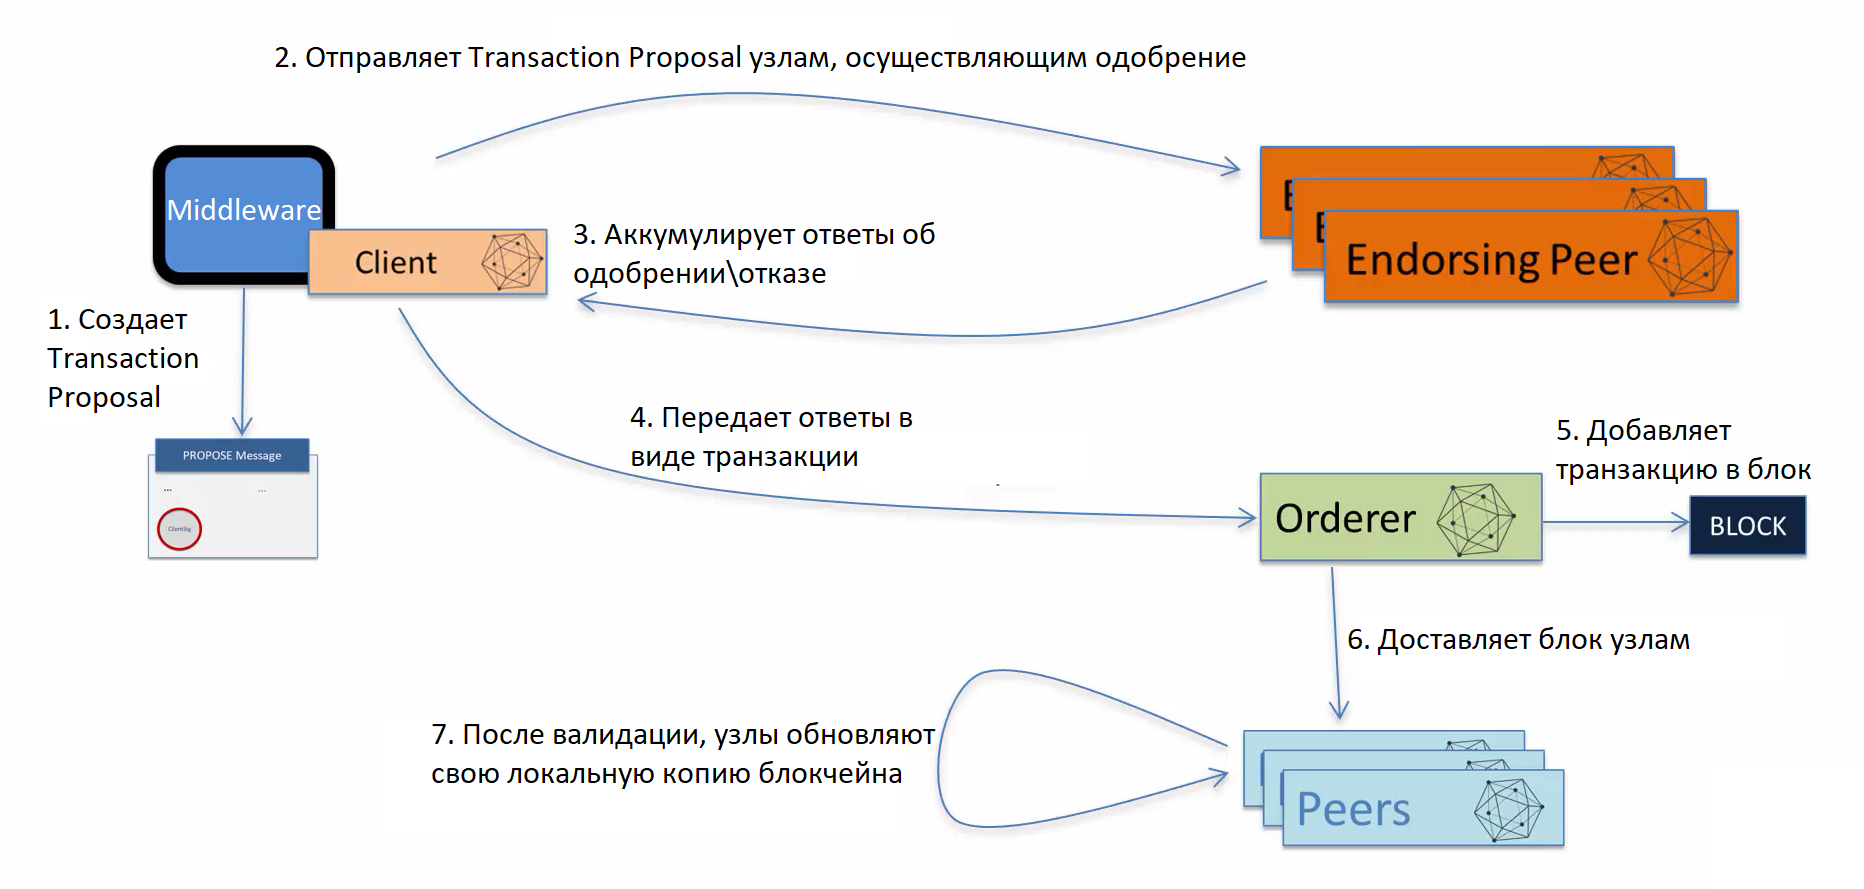
\includegraphics [scale=0.6] {tr-flow}
	\caption{Создание транзакции}
	\label{fig:tr-flow}
\end{figure}

\section{Триллеммы децентрализованных систем} \label{sec:ch1/sec4}
Существует точка зрения насчет распределенных систем, известная “теорема CAP”\cite{cap-t}. Заключается она в утверждении о том, что есть три основных характеристики распределенных систем - доступность(Availability), согласованность(Consistency) и устойчивость к разделению (Partition Tolerance), и гарантия поддержки их всех в принципе невозможна: всегда приходится выбирать две характеристики из эти трех. То есть, речь идет о классификации распределенных систем по степени обладания тем или иным набором свойств. Схематично данное разделение представлено на рисунке \ref{fig:cap_theoreme}. На рисунке выделены три класса: CA, CP и AP.

\begin{figure}[ht]
	\centering
	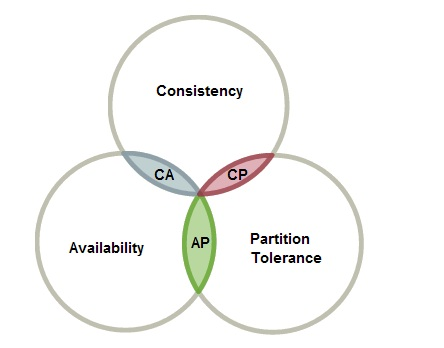
\includegraphics [scale=1.0] {cap-theorem}
	\caption{Визуализация теоремы CAP}
	\label{fig:cap_theoreme}
\end{figure}


Достижение баланса между этими тремя свойствами является задачей первостепенной важности при проектирование распределенной системы.
Фундаментальный компромисс между свойствами, описанный в теореме в большей степени касается систем с распределенной архитектурой, которые развернуты в ненадежных сетях, например в сети Интернет.
Под доступностью мы понимаем то, что при возникновении сбоя в части узлов отказ в обслуживании не происходил для всех пользователей и процессов системы. Их количество должно быть незначительным для поддержания нормальной работоспособности системы. Согласованность же заключается в том, чтобы в системе не происходило искажение данных. 

Архитектура Hyperledger Fabric приближена к классу AP, как и в большинстве других блокчейн платформ. То есть получается что устойчивость к разделению и доступность гарантированы в большинстве блокчейн платформ, в том числе и в Hyperledger Fabric. Возникает вопрос о согласованности и каждая платформа обеспечивает ее по своему, может быть несколько вариантов.   

Таким образом, с точки зрения теоремы CAP, блокчейн-ориентированные системы определяют ее свойства следующим образом:
\begin{itemize}
	\item \textbf{Согласованность} - предотвращение разветвлений цепи блоков.
	\item \textbf{Доступность} - предоставление пользователям информации о транзакциях, записываемых в цепь транзакции, происходит на всех узлах сети.
	\item \textbf{Устойчивость к разделению} - сеть не престает функционировать в случае задержек и сбоев, возникающих в некоторых её частях.
\end{itemize}

С точки зрения свойств CAP Hyperledger Fabric можно рассматривать следующим образом:
\begin{itemize}
	\item \textbf{Согласованность} - порядок транзакций заранее определен, а также управление версиями смарт контрактов происходит с оптимистичным подходом( MVCC)\cite{mvcc}.
	\item \textbf{Доступность} - копия цепи блоков размещается на каждом из узлов.
	\item \textbf{Устойчивость к разделению} - работа бизнес сети не прекращается, в случае возникновения некоторого количества неисправных узлов(порог задается при конкурировании сети).
\end{itemize}

Как уже упоминалось раньше, системы распределенного реестра могут страдать от недостатка согласованности данных и вот как Hyperledger Fabric обеспечивает её:
\begin{itemize}
	\item  В обработке транзакций участвуют несколько компонентов сети и все они проверяют подписи друг друга, а также целостность принятых ими данных.
	\item Инициация транзакций происходит клиентами путем отправки заявки на добавление транзакции, содержащей все необходимые данные осуществляющим одобрение узлам и только после этого они поступают отдельному компоненту, ответственному за создание и распространение блоков по сети.
	\item В сети находится отдельный узел, осуществляющий упаковку транзакций в блоки в едином, гарантированном порядке, и их доставку прочим узлам.Таким образом, порядок транзакций гарантированно согласован по всей
	\item Валидация блока узлом происходит с использованием механизма MVCC. Механизм MVCC гарантирует согласованность полученного блока. В случае не прохождения валидации транзакциям в блокчейне устанавливается соответствующий статус, исходя из которого можно говорит о недействительности транзакций.
	\item Цепь представляет из себя последовательность полностью упорядоченных блоков, где каждый блок содержит транзакций (находящихся в одном из двух статусов, валидная ил не валидная). Таким образом достигается упорядоченность во всей сети.
\end{itemize}

Теорема САР имеет сходство с трилеммой блокчейна, утверждающей о том, что нельзя одновременно достичь идеала по трем параметрам:
\begin{itemize}
	\item Масштабируемость;
	\item Безопасность;
	\item Децентрализация.
\end{itemize}

На рисунке~\ref{fig:trilem-blockchain} цветами отмечены характеристики системы с уклоном в тот или иной параметр:
\begin{itemize}
	\item \textbf{Зеленый:} сбалансированное состояние трех условий;
	\item \textbf{Красный:} сильная безопасность, но ограниченные децентрализация и масштабируемость;
	\item \textbf{Синий:} высокая эффективность, но безопасность и децентрализация ограничены;
	\item \textbf{Черный:} высокая децентрализации, но нет некоторых аспектов масштабируемости и безопасности.
	\item \textbf{Серый:} полная децентрализация, с минимальными или отсутствующими качествами безопасности и масштабируемости.
	\item \textbf{Фиолетовый:} равный баланс между безопасностью и масштабируемостью, отказ от децентрализации.
\end{itemize}

\begin{figure}[ht]
	\centering
	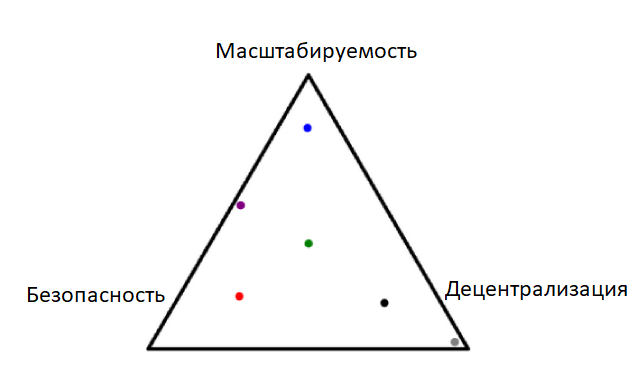
\includegraphics [scale=1.0] {trilem-blockchain}
	\caption{Визуализация трилемммы блокчейна}
	\label{fig:trilem-blockchain}
\end{figure}

Под децентрализацией мы понимаем возможность запускать блокчейн на таких небольших компьютерах, как ноутбуки, сохраняя при этом безопасность даже в случае проведения атаки с превосходящими мощностями. Таким образом поддерживается устойчивость блокчейна к попытке его изменения, одновременно сохраняя возможность быстро и, что немаловажно, одновременно совершать и обрабатывать большое количество (относительно размера сети) транзакций.

В ранних реализациях блокчейна не было уделено должного внимания масштабируемости системы, тогда как в блокчейнах последующих поколения отклоняются от децентрализации в угоду масштабируемости. Не все узлы таких реализаций синхронизируют  свои действия друг с другом, а, например, только некоторое количество самых мощных узлов с высокой пропускной способностью. Так как валидаторов можно сменить путем голосования, сеть всё еще остается децентрализованной.


\section{Постановка задачи} \label{sec:ch1/sec5}
В рамках данной работы требуется реализовать систему электронного документооборота как части инфраструктуры предприятия на примере задачи подписания документов в вузе. Разрабатываемый СЭД должен быть основан на распределенном реестре и иметь клиент в виде мобильного приложения.

Для этого необходимо реализовать следующие задачи:
\begin{enumerate}
	\item Изучить Enterprise-решение Hyperledger Fabric как систему, реализующую технологию распределенных реестров.
	\item Изучить способы построения надежных систем документооборота.
	\item Реализовать бизнес приложение для системы электронного документооборота.
	\item Реализовать интерфейс взаимодействия с бизнес-приложением на основе REST-API.
	\item Реализовать мобильное приложение представляющее возможность взаимодействовать с распределенным реестром посредством графического интерфейса.
\end{enumerate}

Ключевой аспект системы, разработка которой является одной из задач данной работы, - надежность. Этот аспект назван ключевым, так как в области работы с документами высокая защищенность данных является одной из наиболее необходимых характеристик системы. Системы, основанные на блокчейне, по определению имеют хороший уровень безопасности, поэтому в нашем случае цель определяет технологию которую мы используем.